\documentclass[border=12]{standalone}

\usepackage{amsmath}
\usepackage{ifthen}
\usepackage{makecell}
\usepackage{pgfmath}
\usepackage{standalone}
\usepackage{stix}
\usepackage{tikz}
\usepackage{tikz-3dplot}
\usepackage{tkz-euclide}
%
%
%
\usetkzobj{all}
\usetikzlibrary{angles}
\usetikzlibrary{arrows.meta}
\usetikzlibrary{arrows}
\usetikzlibrary{automata}
\usetikzlibrary{calc}
\usetikzlibrary{circuits.logic.IEC}
\usetikzlibrary{circuits.logic.US}
\usetikzlibrary{decorations.footprints}
\usetikzlibrary{decorations.markings}
\usetikzlibrary{decorations.pathmorphing}
\usetikzlibrary{decorations.pathreplacing}
\usetikzlibrary{decorations.shapes}
\usetikzlibrary{decorations.text}
\usetikzlibrary{intersections}
\usetikzlibrary{mindmap}
\usetikzlibrary{patterns}
\usetikzlibrary{positioning}
\usetikzlibrary{quotes}
\usetikzlibrary{shadings}
\usetikzlibrary{shadows}
\usetikzlibrary{shapes.callouts}
\usetikzlibrary{shapes.geometric}
\usetikzlibrary{shapes}

%
\definecolor{Grey}{RGB}{76,76,78}
\definecolor{Blue}{RGB}{85,164,224}
\definecolor{Red}{RGB}{225,75,59}
\definecolor{Green}{RGB}{16,158,36}
\definecolor{Orange}{RGB}{243,162,3}
\definecolor{Purple}{RGB}{124,36,231}
\definecolor{Fushia}{RGB}{225,50,162}
%
\definecolor{Grey1}{RGB}{130,130,131}
\definecolor{Blue1}{RGB}{98,170,223}
\definecolor{Red1}{RGB}{236,98,88}
\definecolor{Green1}{RGB}{105,186,108}
\definecolor{Orange1}{RGB}{251,192,79}
\definecolor{Purple1}{RGB}{160,114,235}
\definecolor{Fushia1}{RGB}{237,97,174}


\begin{document}
	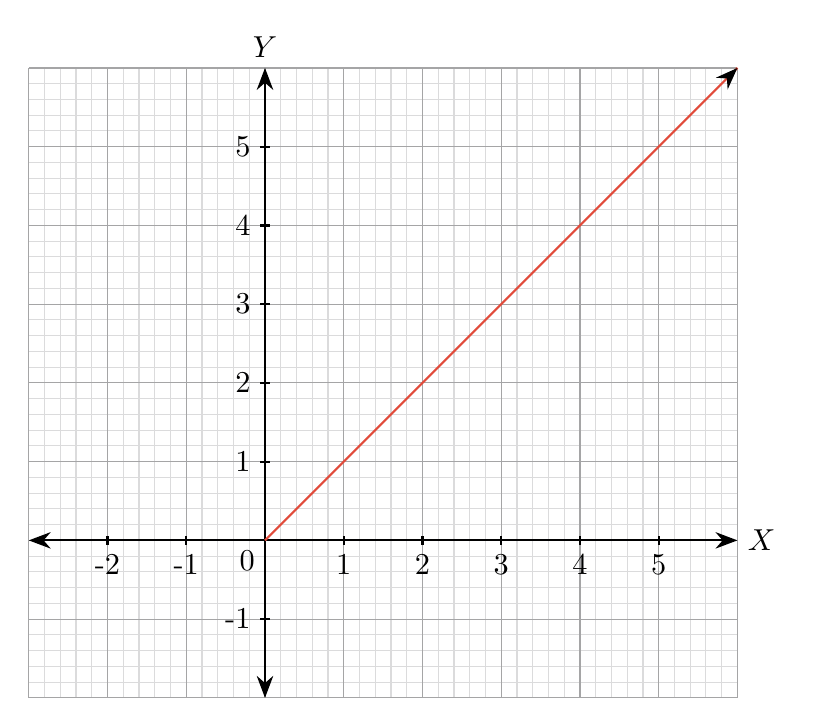
\begin{tikzpicture}
	\begin{scope}[>={Stealth[scale=1.2]}, thick,line join=round, font=\fontsize{11.25}{11.25}\selectfont]
	\pgfgettransformentries{\mya}{\myb}{\myc}{\myd}{\mys}{\myt}
	\pgfmathsetmacro{\preserve}{1/\mya}	

\draw [thin,Grey!20,step=0.2]  (-3,-2) grid (6,6);
\draw [thin,Grey!50,step=1]  (-3,-2) grid (6,6);
\foreach \x in {-2,-1,1,2,...,5}{
	\pgfmathsetmacro{\n}{int(\x)}
	\node at (\x,0) {\tikz{\draw [thick] (0,-0.35ex)--(0,0.35ex);}};
	\node at (\x,-0.35ex) [anchor=north] {
		\nagwaMathLabel
		{\n}};}
\foreach \y in {-1,1,2,...,5}{
	\pgfmathsetmacro{\n}{int(\y)}
	\node at (0,\y) {\tikz{\draw [thick] (-0.35ex,0)--(0.35ex,0);}};
	\node at (-0.35ex,\y) [anchor=east] {
		\nagwaMathLabel
		{\n}};}
\draw [<->] (-3,0)--(6,0) node [anchor=west] {$X$};
\draw [<->] (0,-2)--(0,6) node [anchor=south] {$Y$};
\node [anchor=north east] at (0,0) {$0$};


\draw [Red](0,0)--(6,6);
\path [postaction={decorate, decoration={markings,mark=at position 1 with {\arrow[]{>}}}}](0,0)--(6,6);
	
	\end{scope}
	\end{tikzpicture}
\end{document}